\documentclass{beamer}
%
% Choose how your presentation looks.
%
% For more themes, color themes and font themes, see:
% http://deic.uab.es/~iblanes/beamer_gallery/index_by_theme.html
%
\mode<presentation>
{
  \usetheme{Boadilla}      % or try Darmstadt, Madrid, Warsaw, ...
  \usecolortheme{beaver} % or try albatross, beaver, crane, ...
  \usefonttheme{default}  % or try serif, structurebold, ...
  \setbeamertemplate{navigation symbols}{}
  \setbeamertemplate{caption}[numbered]
  
} 

\usepackage{xcolor,colortbl}
\usepackage[english]{babel}
\usepackage[utf8x]{inputenc}
\usepackage{courier}
\usepackage{dsfont}
\usepackage{verbatim} 
\usepackage{enumerate}
\usepackage{tikz}
\usepackage{multirow}
\usepackage{bbm}
\usepackage{amsmath}
\usepackage{venndiagram}
\usepackage{epigraph} 
%\usepackage{xcolor}

%\usepackage{enumitem}

\usepackage{hyperref}
\hypersetup{
    colorlinks=true,
    linkcolor=blue,
    filecolor=magenta,      
    urlcolor=cyan,
}

% R stuff!
\usepackage{listings}
\definecolor{codegreen}{rgb}{0,0.6,0}
\definecolor{codegray}{rgb}{0.5,0.5,0.5}
\definecolor{codepurple}{rgb}{0.58,0,0.82}
\definecolor{backcolour}{rgb}{0.95,0.95,0.92}

\lstdefinestyle{mystyle}{
    backgroundcolor=\color{backcolour},    
    commentstyle=\color{codegreen},
    keywordstyle=\color{black},
    numberstyle=\tiny\color{codegray},
    stringstyle=\color{codepurple},
    basicstyle=\ttfamily\footnotesize,
    breakatwhitespace=false,         
    breaklines=true,                 
    captionpos=b,                    
    keepspaces=true,                 
    numbers=left,                    
    numbersep=5pt,                  
    showspaces=false,                
    showstringspaces=false,
    showtabs=false,                  
    tabsize=2
}

\lstset{style=mystyle}



%% Size options for nested itemized lists
\usepackage{relsize}
\setbeamerfont{itemize/enumerate body}{parent=normal text}
\setbeamerfont{itemize/enumerate subbody}{parent=normal text,size=\relsize{-1}}
%\setbeamerfont{itemize/enumerate subsubbody}{parent=normal text,size=\relsize{-1}}




\setbeamertemplate{enumerate items}[default]
\setbeamertemplate{itemize item}[triangle]

%\setitemize{label=\usebeamerfont*{itemize item}%
%  \usebeamercolor[fg]{itemize item}
%  \usebeamertemplate{itemize item}}


\usetikzlibrary{shapes,decorations,arrows,calc,arrows.meta,fit,positioning}
\tikzset{
    -Latex,auto,node distance =1 cm and 1 cm,semithick,
    state/.style ={ellipse, draw, minimum width = 0.7 cm},
    point/.style = {circle, draw, inner sep=0.04cm,fill,node contents={}},
    bidirected/.style={Latex-Latex,dashed},
    el/.style = {inner sep=2pt, align=left, sloped}
}

\newcommand{\Mypm}{\mathbin{\tikz [x=1.4ex,y=1.4ex,line width=.1ex] \draw (0.0,0) -- (1.0,0) (0.5,0.08) -- (0.5,0.92) (0.0,0.5) -- (1.0,0.5);}}%



%% For block quote
\usepackage{etoolbox}
\AtBeginEnvironment{quote}{\par\singlespacing\small}


\title[STA-209]{Inference for Linear Regression}
\subtitle{ANOVA for SLR}
%\author{}
\author{Grinnell College}
\date{December 6, 2024}

\graphicspath{{img/}}

\begin{document}

\begin{frame}
  \titlepage
\end{frame}

\begin{frame}{Review}

\begin{itemize}
\item Hypothesis testing
\begin{itemize}
    \item test-statistics
    \item p-values
    \item need to be careful what $H_0$ and $H_A$ actually are
\end{itemize} \vspace{4mm}

\item ANOVA
\begin{itemize}
    \item testing equality of group means
    \item $H_0$: $\mu_1 = \mu_2 = \dots = \mu_k$
    \item F = $\frac{MSG}{MSE} = \frac{SSG/(k-1)}{SSE/(n-k)}$
    \item MSG measures how far (on average) group means are from overall mean
    \item MSE measures how far (on average) observations are from their group means
\end{itemize}
\end{itemize}
\end{frame}



\begin{frame}{ANOVA and Regression}

ANOVA Null hypothesis:

\begin{align*}
H_0: \mu_1 = \mu_2 = \dots \mu_k
\end{align*}

\begin{itemize}
    \item comparing mean values of a continuous variable for $k$ different groups
    \item $H_0$ true $\implies$ each group has same \textit{overall} mean $\mu$
\end{itemize} \vspace{8mm}

We are going to see how this ANOVA stuff can be applied to linear regression
\end{frame}

\begin{frame}{ANOVA and Regression}

We might ask if it is better to predict an outcome ($\hat{y}$) using an overall mean or if we are better off predicting with a group mean:

\begin{align*}
H_0: \hat{y}_{j} = \mu, \qquad H_A: \hat{y}_j = \mu_j
\end{align*} \vspace{6mm}

In this case by \textit{better}, we mean that we minimize the residual sum of squares, or the squared difference between our prediction and the true value
\begin{align*}
\text{Sums of Squared Residuals} &= \sum_{i=1}^n (y_i - \hat{y}_i)^2 \\
&= \sum_{i=1}^n e_i^2
\end{align*}

% \begin{itemize}
%     \item goal: to minimize SSR, we need to find a good way to predict $y_j$
%     \item in this scenario we are comparing predictions using $\hat{y}_j = \mu$ and $\hat{y}_j = \mu_j$
% \end{itemize}

\end{frame}

\begin{frame}{Regression}
Recall that regression formulas are of the form:

\begin{align*}
y_i = \beta_0 + X_i \beta_1 + \epsilon_i
\end{align*}

\begin{itemize}
    \item $\beta_0$ represents an intercept
    \item $\beta_1$ indicates a slope associated with $X_i$
\end{itemize} \vspace{12mm}

Once we fit to line to the data, we have an estimated line of
\begin{align*}
\hat{y}_i = \hat{\beta}_0 + X_i \hat{\beta}_1 \hspace{2mm} (= b_0 + b_1X_i)
\end{align*}

\begin{itemize}
    \item residual $e_i = y_i - \hat{y}_i$ is an estimate of the error $\epsilon_i$
\end{itemize}
\end{frame}

\begin{frame}{\texttt{mpg} Example}
Consider the \texttt{mpg} dataset, where we might be interested in estimating the city miles per gallon of various vehicles

\begin{center}
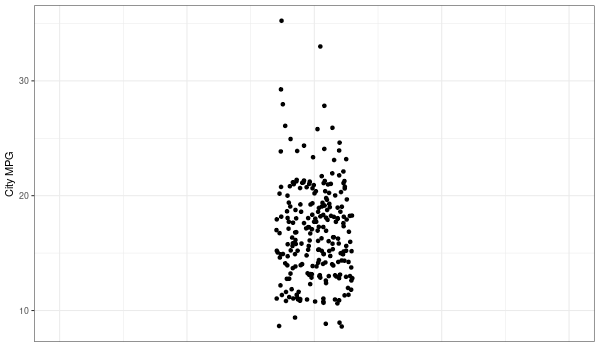
\includegraphics[scale=0.5]{ctympg0.png}
\end{center}

\end{frame}

\begin{frame}{mpg Example}
\small
Using simply the overall mean, we would have total squared error of 4220

\begin{center}
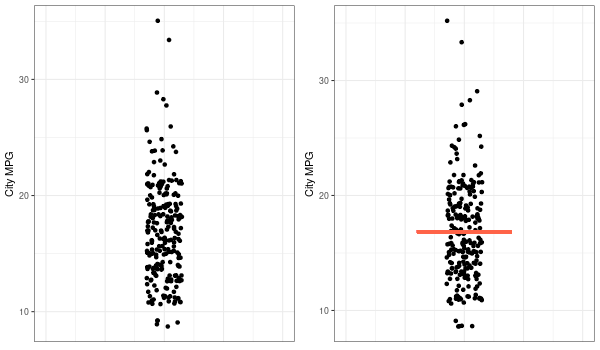
\includegraphics[scale=0.45]{ctympg1.png}
\end{center}
% latex table generated in R 4.4.0 by xtable 1.8-4 package
% Sun Apr 28 14:46:06 2024
\begin{table}[ht]
\centering
\begin{tabular}{lrrrrr}
  \hline
 & Df & Sum Sq & Mean Sq & F value & Pr($>$F) \\ 
  \hline
Residuals   & 233 & 4220.35 & 18.11 &  &  \\ 
   \hline
\end{tabular}
\end{table}
\end{frame}

\begin{frame}{mpg Example}
\footnotesize
Consider the alternative, where we predict city mileage based on drive train
\begin{center}
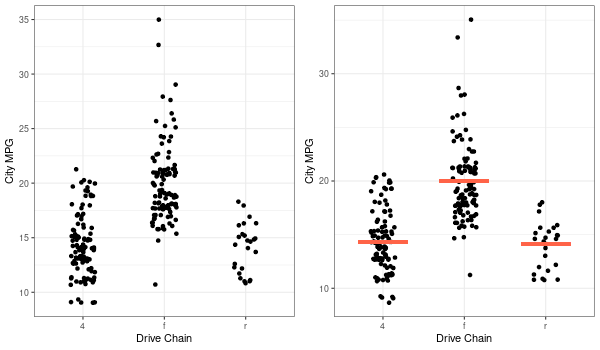
\includegraphics[scale=0.44]{ctympg2.png}
\end{center}
% latex table generated in R 4.4.0 by xtable 1.8-4 package
% Sun Apr 28 14:48:09 2024
\begin{table}[ht]
\centering
\begin{tabular}{lrrrrr}
  \hline
 & Df & Sum Sq & Mean Sq & F value & Pr($>$F) \\ 
  \hline
drv         & 2 & 1878.81 & 939.41 & 92.68 & $<$0.0001 \\ 
  Residuals   & 231 & 2341.53 & 10.14 &  &  \\ 
   \hline
\end{tabular}
\end{table}
\begin{itemize}
    \item SSR has gone down (good!) and is sequestered into SSG (drv)
\end{itemize}
\end{frame}

\begin{frame}[fragile]{mpg Example}
In terms of a regression model, we could frame this as

\begin{align*}
\hat{y} = \mathbbm{1}_{\text{4wd}} \hat{\beta}_1 + \mathbbm{1}_{\text{Fwd}} \hat{\beta}_2 + \mathbbm{1}_{\text{Rwd}} \hat{\beta}_3
\end{align*}

where $\mathbbm{1}$ represents our \textit{indicator variable} and, in the case of categorical variable regression, $\hat{\beta}$ represents the mean value for each group. This is exactly what we saw towards the beginning of the semester \vspace{2mm}

\begin{lstlisting}[language=R]
> lm(cty ~ -1 + drv, mpg)

Coefficients:
 drv4   drvf   drvr  
14.33  19.97  14.08  
\end{lstlisting}
\begin{center}
$\hat{y} = (14.33 \times \mathbbm{1}_{\text{4wd}})  + (19.97 \times \mathbbm{1}_{\text{Fwd}})  + (14.08 \times \mathbbm{1}_{\text{Rwd}})$
\end{center}

\end{frame}

\begin{frame}[fragile]{Baseline Category}
\small
By default, R will choose one category as the ``reference" variable
\begin{itemize}
    \item usually based on 1st alphabetic category or lowest numeric
\end{itemize}

\begin{lstlisting}[language=R]
> lm(cty ~ drv, mpg)
(Intercept)         drvf         drvr  
    14.3301       5.6416      -0.2501  
\end{lstlisting} \vspace{-4mm}

\begin{align*}
\hat{y} = \hat{\beta}_0 + \mathbbm{1}_{\text{Fwd}} \hat{\beta}_1+ \mathbbm{1}_{\text{Rwd}} \hat{\beta}_2 = 14.33 + 5.64 \times \mathbbm{1}_{\text{Fwd}} - 0.25 \times \mathbbm{1}_{\text{Rwd}}
\end{align*}

\begin{center}
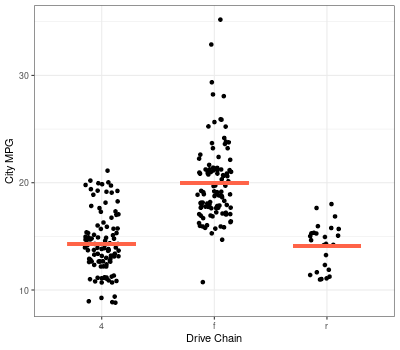
\includegraphics[scale=0.37]{ctympg3.png}
\end{center}

\end{frame}


\begin{frame}{Inference and Regression}
So, what we have just seen tells us:
\begin{itemize}
    \item SLR with one categorical variable as a predictor is actually a special case of ANOVA
    \item both attempted to minimize SSE (=SSR) by partioning that variance into something else (SSG)
\end{itemize} \vspace{10mm}

However, instead of simply assessing whether or not there is \textit{any} difference between groups, we may be interested specifically in estimating values of $\beta$ in the expression \vspace{-4mm}

\begin{align*}
y = \beta_0 + X \beta_1 + \epsilon
\end{align*}
where X is a \textit{quantitative} variable
\end{frame}

\begin{frame}{Inference and Regression}
\begin{align*}
y = \beta_0 + \beta_1X + \epsilon
\end{align*}

When considering a regression line, we are actually trying to find out if there is a linear relationship between the variables. \vspace{6mm}

We could test this by structuring a null hypothesis like so: \vspace{-4mm}

\begin{align*}
H_0: \hspace{1mm} &\text{there is no linear relationship} \\
(\text{equivalently}) \hspace{4mm} H_0: \hspace{1mm} &\beta_1 = 0\\
\end{align*}

Given our estimate of $\hat{\beta}$, we can make the test statistic, 

\begin{align*}
t = \frac{\hat{\beta}_1}{SE_{\beta_1}}
\end{align*}
\end{frame}



\begin{frame}[fragile]{mpg Example}

Comparing residuals and F statistic for ANOVA and regression

\begin{lstlisting}[language=R]
> aov(cty ~ drv, mpg) %>% summary()
             Df Sum Sq Mean Sq F value Pr(>F)    
drv           2   1879   939.4   92.68 <2e-16 ***
Residuals   231   2342    10.1                   

\end{lstlisting}
\begin{lstlisting}[language=R]
> lm(cty ~ drv, mpg) %>% summary() 

Coefficients:
            Estimate Std. Error t value Pr(>|t|)    
(Intercept)  14.3301     0.3137  45.680   <2e-16 ***
drvf          5.6416     0.4405  12.807   <2e-16 ***
drvr         -0.2501     0.7098  -0.352    0.725    


Residual standard error: 3.184 on 231 degrees of freedom
Multiple R-squared:  0.4452,	Adjusted R-squared:  0.4404 
F-statistic: 92.68 on 2 and 231 DF,  p-value: < 2.2e-16
\end{lstlisting}

\end{frame}


\begin{frame}[fragile]{mpg Example}

Comparing pairwise differences for TukeyHSD and regression (reference/intercept variable is 4WD)

\begin{lstlisting}[language=R]
> aov(cty ~ drv, mpg) %>% TukeyHSD()
  Tukey multiple comparisons of means
    95% family-wise confidence level

          diff       lwr       upr     p adj
f-4  5.6416010  4.602497  6.680705 0.0000000
r-4 -0.2500971 -1.924554  1.424359 0.9338857
r-f -5.8916981 -7.561520 -4.221876 0.0000000
\end{lstlisting}
\begin{lstlisting}[language=R]
> lm(cty ~ drv, mpg) %>% summary() 

Coefficients:
            Estimate Std. Error t value Pr(>|t|)    
(Intercept)  14.3301     0.3137  45.680   <2e-16 ***
drvf          5.6416     0.4405  12.807   <2e-16 ***
drvr         -0.2501     0.7098  -0.352    0.725    

\end{lstlisting}

\end{frame}

\begin{frame}{ANOVA and Regression}

ANOVA is a generalization of the t-test for multiple groups
\begin{itemize}
    \item regression is a generalization of ANOVA for any combination of variables
    \item only tells us that a difference exists, not \textit{what} the difference actually is
\end{itemize} \vspace{10mm}

Benefits of Regression:
\begin{itemize}
    \item requires fewer assumptions about data
    \begin{itemize}
        \item ANOVA has a hidden assumption of Normal groups
    \end{itemize}
    \item provides statistical tests for each of the group categories
    \item allows us to predict quantitative outcome using a quantitative predictor
\end{itemize}
\end{frame}

\begin{frame}{Regression Example}
Which of these do you suspect will have the smallest residual error?
\begin{itemize}
    \item think about how far observations are from predictions
\end{itemize}
\begin{center}
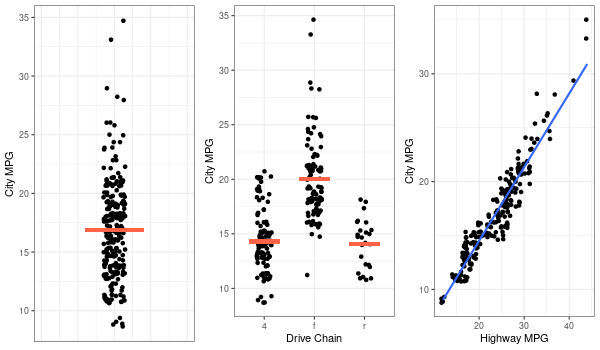
\includegraphics[scale=0.55]{ctympg4.png}
\end{center}
\end{frame}


\begin{frame}[fragile]{mpg Example}

\begin{lstlisting}[language=R]
> lm(cty ~ hwy, mpg) %>% summary()


Coefficients:
            Estimate Std. Error t value Pr(>|t|)    
(Intercept)  0.84420    0.33319   2.534   0.0119 *  
hwy          0.68322    0.01378  49.585   <2e-16 ***


Residual standard error: 1.252 on 232 degrees of freedom
Multiple R-squared:  0.9138,	Adjusted R-squared:  0.9134 
F-statistic:  2459 on 1 and 232 DF,  p-value: < 2.2e-16
\end{lstlisting} \vspace{-4mm}


\begin{align*}
\hat{y} = b_0 + b_1 \times (hwy) = 0.84 + 0.68 \times (hwy)
\end{align*} \vspace{-4mm}

\begin{itemize}
    \item F is testing whether both intercept and slope are zero
    \item t is testing for specifically slope/intercept one at a time
    \item it is possible that the F-test shows a linear model works well, but that the intercept is not significant
\end{itemize}
\end{frame}

\begin{frame}{Interpretations}
Interpretations of coefficients is exactly the same as before: \vspace{4mm}

\textbf{Slope (b$_1$):} how much the prediction for y ($\hat{y}$) changes when we change the X variable \vspace{2mm}

\textbf{Intercept (b$_0$):} our prediction for y ($\hat{y}$) when X = 0 \vspace{14mm}

MPG example: $\widehat{city} = b_0 + b_1 \times (hwy) = 0.84 + 0.68 \times (hwy)$ \vspace{2mm}

\textbf{Slope:}
\begin{itemize}
    \item when we change the hwy mpg of a vehicle by 1, the predicted city mpg changes by 0.68
\end{itemize} \vspace{2mm}

\textbf{Intercept:}
\begin{itemize}
    \item when the highway mpg of a vehicle is 0, the predicted city mpg is 0.84
\end{itemize}
    
\end{frame}


\begin{frame}{Key Takeaways}
\begin{itemize}
\item Regression is a generalization of ANOVA
\item The $\beta$ coefficients indicate how much a change in $X$ impacts a change in $Y$
\item Under the null, $H_0: \beta = 0$ 
\item $R^2$ gives an estimate of explained variance that, in the case of regression with a categorical variable, is identical to the sum of between-group variability
\item Likewise, the residuals correspond to the total within-group variability
\end{itemize}
\end{frame}

%\begin{frame}
%\begin{columns}
%
%  \begin{column}{0.45\textwidth}
%%
%  \end{column}
%  \begin{column}{0.45\textwidth}
%%
%  \end{column}
%
%\end{columns}
%\end{frame}


\end{document}
